% V 2024 09 30
\documentclass{article}
\usepackage[utf8]{inputenc}
\usepackage[T1]{fontenc}
\usepackage[magyar]{babel}
\usepackage[dvipsnames,svgnames,x11names]{xcolor}
\usepackage{graphicx}
\usepackage{caption}
% Ezeket a preambulumban kell megadni!
\DeclareCaptionFont{pirosszamok}{\color{red}}
\DeclareCaptionFont{kekszoveg}{\color{blue}}
%opening
\title{Kép- és egyéb feliratok felturbózása,\\ a \texttt{caption} csomag}
\author{Virágh János}
% egyebek
\setlength{\parindent}{0pt}
%
\begin{document}
\maketitle
\tableofcontents
\listoftables
\listoffigures

\section{Játék az aláírásokkal}
A \texttt{babel} csomag a \texttt{magyar} opcióval az úsztatott objektumokhoz (képek, táblázatok) általában a tipográfiai szokásoknak megfelelő, korrekt formázású feliratokat biztosít, amelyeket rendszerint a képek \emph{alatt} és a táblázatok \emph{fölött} helyezünk el. Ha ezen túl még valamin változtatni szeretnénk, a \texttt{caption} csomag számos alternatívát kínál.
\subsection{Elnevezések módosítása}
Ha nem tetszik az ábrafeliratokban a  Babel csomag magyar opciója által felkínált ,,ábra'' kifejezés, például így módosíthatjuk:

\begin{verbatim}
\captionsetup[figure]{name=kép}
\end{verbatim}
\captionsetup[figure]{name=kép}

\noindent  Figyeljük meg, hogyan változnak az aláírások.
\begin{figure}[!htp]
  \begin{center}
   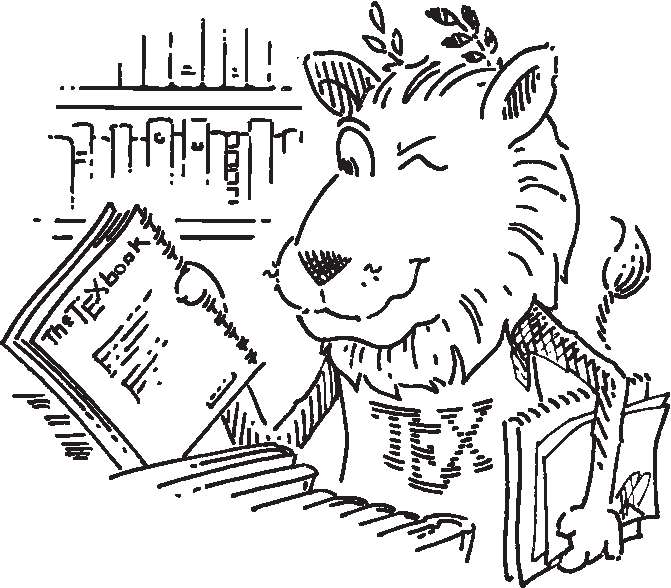
\includegraphics[scale=0.25]{Lion.pdf}
  \caption{Kedvenc oroszlánunk}
  \label{abra-oroszlanori}
  \end{center}
\end{figure}
\Aref{abra-oroszlanori}.~ábrán kedvenc oroszlánunkat látjuk.

\noindent Legyen még egy kép, más nézetből! De most változtassuk az aláírást ,,fotó''-ra a
\begin{verbatim}
\captionsetup[figure]{name=fotó}
\end{verbatim}
\captionsetup[figure]{name=fotó}
paranccsal:
\begin{figure}[hbp]
  \begin{center}
    \reflectbox{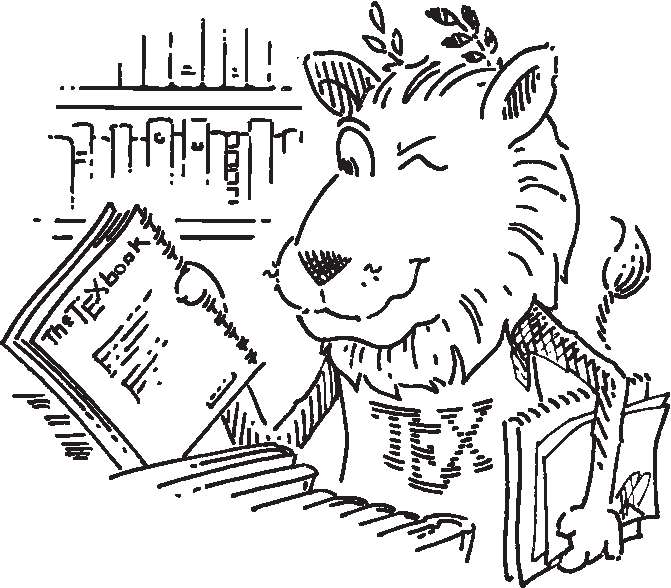
\includegraphics[scale=0.25]{Lion.pdf}}
  \end{center}
  \caption{Kedvenc oroszlánunk a tükörben}
\end{figure}

\subsection{Színezett aláírások}
A \verb!caption! csomaggal sokkal többet is elérhetünk. Egy példa:
a preambulumban(!) megadott
\begin{verbatim}
\DeclareCaptionFont{pirosszamok}{\color{red}}
\DeclareCaptionFont{kekszoveg}{\color{blue}}	
\end{verbatim}
utasítások után a főszövegben kiadható a
\begin{verbatim}
\captionsetup{labelfont={pirosszamok,bf},textfont=kekszoveg}
\end{verbatim}
\captionsetup{labelfont={pirosszamok,bf},textfont=kekszoveg}
utasítás, ami után   \apageref{figure-dizzylion}.~oldali \ref{figure-dizzylion}.~ábrán látható szép csicsás aláírást kapjuk.

\begin{figure}[!hbp]
  \begin{center}
    \rotatebox{45}{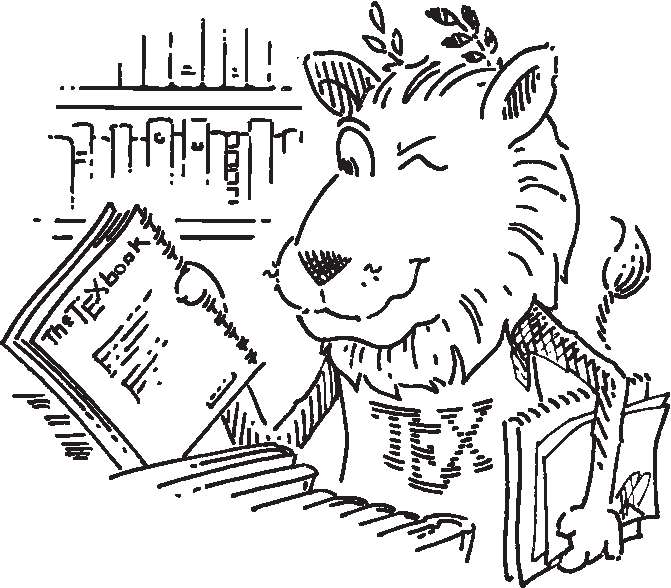
\includegraphics[scale=0.25]{Lion.pdf}}
  \end{center}
  \caption{Kedvenc oroszlánunk szédül}
  \label{figure-dizzylion}
\end{figure}

További elrettentő példák a \verb!caption-eng-new.pdf! kézikönyvben.

\textbf{Megjegyzés}. Előfordulhat, hogy némelyik opció összeakad a \verb!babel! csomag magyar nyelvi támogatásával, ugyanis abban is vannak a magyar nyelv sajátosságai miatt a föliratokra vonatkozó egyedi trükközések.

Az úsztatott  táblázatokra is alkalmazhatók hasonló trükkök, például a
\begin{verbatim}
\captionsetup{labelfont={pirosszamok,bf},textfont={pirosszamok,it}}
\end{verbatim}
\captionsetup{labelfont={pirosszamok,bf},textfont={pirosszamok,it}}
parancs kiadása után \aref{table-kicsi}.~táblázat felett szép, tisztapiros feliratot látunk. ;-)
\begin{table}[htp]
 \caption{Egyszerű $3\times3$-as táblázat}	
 \label{table-kicsi}
  \begin{center}
    \begin{tabular}{| l c r |}
    \hline
    1 & 2 & 3 \\
    4 & 5 & 6 \\
    7 & 8 & 9 \\
    \hline
    \end{tabular}
  \end{center}
\end{table}
%
\end{document}
